\documentclass[12pt]{article}

\usepackage{fullpage}
\usepackage{graphicx}
\usepackage{graphics}
\usepackage{mdwlist}
\usepackage{amssymb}
\usepackage{algorithm}
\usepackage{algpseudocode}
\usepackage{algorithmicx}

\setlength{\oddsidemargin}{0.0in}
\setlength{\evensidemargin}{0.0in}
\setlength{\textwidth}{6.5in}
\setlength{\headheight}{0.0in}
\setlength{\topmargin}{0.0in}
% \setlength{\textheight}{9.0in}
\setlength{\textheight}{9in}
\addtolength{\textheight}{-\topmargin}
\addtolength{\textheight}{-\headheight}
\addtolength{\textheight}{-\headsep}
\addtolength{\textheight}{-\footskip}



\begin{document}

\newcommand{\beq}{\begin{equation}}
\newcommand{\eeq}{\end{equation}}
\newcommand{\bit}{\begin{itemize*}}
\newcommand{\eit}{\end{itemize*}}
\newcommand{\goal}[1]{ {\noindent {$\Rightarrow$} \em {#1} } }
\newcommand{\hide}[1]{}
\newcommand{\comment}[1]{ {\footnotesize {#1} } }
\newtheorem{lemma}{Lemma}
\newtheorem{theorem}{Theorem}
\newtheorem{proof}{Proof}
\newtheorem{defn}{Definition}
\newtheorem{algo}{Algorithm}
\newtheorem{observation}{Observation}

\title{Multilevel Approach on Partitioning Real World Graphs}


\author{ {\em Yonwoo Choi} \\
	    Dept. of Computer Science\\
	    Seoul National University\\
	    {\tt yhugestar@snu.ac.kr}
	 \and
	 {\em Hyoyoung Lho} \\
	    Dept. of Computer Science\\
	    Seoul National University\\
	     {\tt hyolho@dbs.snu.ac.kr}
	 \and
	 {\em Sohyun Kim} \\
	    Dept. of Computer Science\\
	    Seoul National University\\
	      {\tt chloek409@dbs.snu.ac.kr}
        }


\maketitle
\begin{abstract}
    In recent years, real world graphs have emerged and are growing exponentially. To analyze real world graphs, partitioning them into smaller groups is necessary due to its massive size in terms of memory and computational power consumption. Therefore, how can we cut them \textit{fast} and \textit{nicely}? We built a method to partition the real world graph data by combining \textit{label propagation} algorithm and \textit{Kernighan-Lin} algorithm. As the experiment result shows, the pipeline of these two algorithms results in faster running time of graph partitioning than using only one method.
\end{abstract}

\section{Introduction}
    \label{sec:intro}
    Graph partitioning problem can be applied in many real world applications, such as VLSI circuit design, internet router design, community detection in SNS and many others. \\ As there are increasing attempts to apply graph partitioning algorithms to real world graphs, many approximate solutions have been developed including multilevel approach and spectral clustering, but there are still no `good cuts'. We therefore propose an iterative multilevel $k$-way graph partitioning algorithm that finds better cuts than the existing schemes.\\
To help you understand the defined problem we are trying to solve, we add a brief explanation of the existing graph partitioning methods. For the rest of the paper, we utilize some general symbols related to graph theory. Table \ref{tab:symbols} gives a list of common symbols we used. \\

\begin{table}[htb]
\begin{center}
\begin{tabular}{|l | c | } \hline \hline
Symbol & Definition \\ \hline
$G = (V,E)$ & graph \\
$n = |V|$ & number of nodes of G \\
$V$ & vertices \\
$E$  & edges \\ 
\hline
\end{tabular}
\end{center}
\caption{Symbols and definitions}
\label{tab:symbols}
 \end{table}


\textbf{1. Existing Methods}\\ \\
Graph partitioning has a clear objective and a clear constraint. The goal is to minimize the edge-cut, and the constraint involves that the sum of the node weights in each partition should be of same size. Choosing optimal methods is an NP-complete problem and thus, we need good heuristics to efficiently obtain high-quality partitions.\\ \\

\rmfamily{1.1 Geometric Partitioning}\\\\
We now describe one of the partitioning algorithm, geometric based algorithm suggested by Miller, Teng, Thruston, and Vavasis. This method uses $circles$ instead of a line to cut the graph. This method is one of the vertex separator, that regards graphs as a collection of vertices, instead of edges. Then when we embed the vertices into d-dimensional space, each vertex will have their unique coordinates. Compute the $centerpoint$ of the projected points on the surface of the $d+1$ dimensional sphere and move the centerpoint to the origin of the sphere. After few more steps of this algorithm yields a vertex separator. \\\


\rmfamily{1.2 Spectral Partitioning} \\\\
Before we get into spectral partitioning, we introduce Laplacian matrices and the Fiedler vector. The Laplacian matrix is defined as $L = D - A$, where $A$ $\subset \mathbb{R}^{n\times n}$ is the adjacency matrix of the graph $G = (V,E)$ and the diagonal matrix $D = diag(Ae)$, where vector $e = (1,1,...1)^{T}$. A Fiedler vector is an eigenvector corresponding to the second smallest eigenvalue of the Laplacian matrix of $G$. Let us assume that $\vec{u} = (u_1, u_2, ..., u_n)$ be a Fiedler vector of the Laplacian of $G$. The idea of spectral partitioning is to find a splitting value $s$ and partition the vertices of $G$ into the set of $i$ such that $u_i > s$ and the set such that $u_i \leq s$.
\\\\
\textbf{2. Overview of Multi-level Partitioning (MLP)} \\\\
Many previous research has been done on MLP to solve the efficiency of large graph partitioning problem. The first step of MLP is to replace $G(V,E)$ by a coarse approximation $G_c(V_c,E_c)$, and partition the coarsened $G_c$ instead. Next we use the partitions of $G_c$ to get a rough partitioning of the original $G$, and then iteratively improve it. Below are detailed explanations of the three stages of MLP: \textbf{coarsening, partitioning, and uncoarsening}.      
\\\\
\rmfamily{2.1 Coarsening Methods} \\ \\
In the first phase, starting with the original graph $G_0$, a sequence $L=<G_0,G_1,\dots,G_m>$ is generated such that $|V_0| > |V_1| > \dots >|V_m|$. At each step, the coarsening algorithm reduces the number of vertices of a graph to form a collapsed vertex of the coarser graph and there are various methods for the reduction. \\
\begin{itemize}
    \item RM (Random Matching)\\
    While randomly visiting all vertices of the given graph and if a vertex \textit{u} has not been matched to another vertex yet, then you randomly select one of its unmatched adjacent vertices. Then you include the edge $(u, v)$ in the matching and mark \textit{u} and \textit{v} as matched. If there is no unmatched adjacent vertex \textit{v}, then vertex \textit{u} remains unmatched.
    \item HEM (Heavy Edge Matching) \\
    Instead of randomly matching a vertex with one of its adjacent unmatched vertices, it is matched with a vertex such that the weight of the edge is heaviest over all valid incident edges. Simply put, the goal of this technique is finding a maximal matching that contains edges with large weight. \\
\end{itemize}
\rmfamily{2.2 Partitioning Algorithms}
\begin{itemize}
    \item Kernighan-Lin Algorithm (KL)\\
    KL is a greedy partition algorithm that takes in a graph containing nodes and vertices as input, and outputs separate subsets that are connected together in an optimal matter. The algorithm optimizes the partition in an iterative manner. Given $G = (N,E,W_E)$, a partitioning $N = A \cup B$, where $|A| = |B|$ and $T=cost(A,B)$, we first find subsets $X$ of $A$ and $Y$ of $B$ with $|X|= |Y|$. Then we consider swapping X and Y if it decreases cost. newA = (A-X) $\cup$ Y and newB = (B-Y) $\cup$ X, newT = cost(newA,newB) $<$ T = cost(A,B). Finally we iteratively repeat the process and compute new T efficiently for many possible X and Y. The KL algorithm is generally robust but it is computationally intensive with a time complexity of $O(|N|^{3})$, shows weak performance with weighted graphs, and due to its randomness, the solution is largely dependant on the first swap. \\
    \item Fiduccia-Mattheyses (FM) \\
    FM works similar to KL but instead of swapping two vertices, KL only swaps a single element every step. FM improved the definitions in KL and the time complexity of the procedure. The gains are computed for single vertex moves in FM compared to exchanges, and the worst case running time of the procedure was reduced to $O(E)$ with new definition and the use of novel data structures. An important advantage of FM is that we are able to convert the gain definition to the case of vertex separators. The move of a vertex can be defined to be from the separator to a partition. We introduce a modification of the FM algorithm in the Proposed Methods section. \\
\end{itemize}
\rmfamily{2.3 Uncoarsening phase} \\
The uncoarsening phase is responsible for projecting back the partition $P_m$ to the original
graph. This is performed in successive projections to finer graphs in the sequence of
$G_{m-1},\dots,G_0$ until the partition on the original graph is obtained.
Computing $P_{i}$ from $P_{i+1}$ is straightforward: $\forall u \in V_i^v
P_i[u] = P_{i+1}[v]$. We simply map the partition of a collapsed vertex to its constituent vertices during a projection. In the process, $P_i$ usually ceases to be locally optimum since it has more vertices and edges.  The refinement algorithms are usually a kind of gain heuristic or a hybrid of gain heuristic and another improvement algorithm. The ones we have seen to be practical are usually implementations based on the Fiduccia-Mattheyses (FM) variant of Kernighan-Lin (KL) optimization algorithm.

\section{Survey}
    \label{sec:survey}
    Next we list the papers that each member read, along with their summary and critique.

\subsection{Papers read by Yonwoo Choi}
The first paper was the Fast and High Quality Multilevel Scheme for Partitioning Irregular Graphs paper by Karypis. 
\cite{Irregular_Graphs}
\begin{itemize*}
\item {\em Main idea}: \\
Deriving three phases of a multilevel algorithm consisted of coarsening, partition of the coarsest graph, and refinement to solve the bottleneck problem which occurs when large graph partitioning is being solved in parallel. For computing fill-reducing orderings for sparse matrices, the algorithm in the paper outperforms previous state of art minimum degree algorithms due to the better global view of the graph, critical for partitioning large graphs.    
\item {\em Use for our project}:\\
It is somewhat related to our project, because there are detailed implementations of the coarsening,uncoarsening which helps provide a good global and local view of the large graph. There are also refinement methods during the uncoarsening phase which can be used to filter outliers from our network. 
\item {\em Shortcomings}:\\
For partitioning the coarsest graph, using spectral bisection nearly has no advantage over previous partitioning methods.  
\end{itemize*}

The second paper was the Balanced Graph Partitioning paper by Andreev. 
\cite{BalancedGraphPartitioning}
\begin{itemize*}
\item {\em Main idea}: \\
Using a bi-criteria approximation algorithm and t-partitioning, it solves the (k, 1+$\epsilon$) balanced partitioning problem. It turns out that this algorithm's running time achieves a polynomial time of $O(log^{2}n)$ in respect to the capacity of edges between different partitions. This algorithm is also capable of balancing the weight of the nodes in the case where nodes of the graph are weighted.
++\item {\em Use for our project}: \\
It is quite related to our project, because we can generalize the $k$ balanced partitioning problem in the paper to the problem to the case where different partitions are required to have different size. Then, we could apply the updated solution for improving the speed of the processor in partitioning graphs.  
\item {\em Shortcomings}: \\
The algorithm requires all partitions have the same size which may not be a general solution to real graphs. 
\end{itemize*}

The third paper was the How to Partition a Billion-Node Graph by Wang.
\cite{Billion_Node_Graph}
\begin{itemize*}
\item {\em Main idea}: \\
Proposes a novel approach called MLP(Multi-level label propagation) method to solve the problem of partitioning billion-node graphs on a general purpose distributed memory system. This approach iteratively coarsens a graph until the graph is small enough to use the METIS\cite{Metis} algorithm to generate the final partitioning on the coarsened graph. Compared to existing methods, MLP is more effective, parallelized, and able to process larger graphs. 
\item {\em Use for our project}: \\
It is highly related to our project, because we are working on partitioning real world graphs using a multi-level approach. The MLP pipeline could be used as a baseline of our approach, and it would be meaningful if we improve the coarsening step or the refinement step with additional constraints. 
\item {\em Shortcomings}:\\
MLP's coarsening strategy convergences quite slow compared to SHEM (Sorted Heavy Edge Matching). If there is a constraint that pays special attention to matching small-degree vertices, there may have been a faster convergence.  
\end{itemize*}


\subsection{Papers read by Hyoyoung Lho }
The first paper was the Graphchi : Large-Scale Graph Computation on Just a PC paper by Kyrola, Blelloch and Guestrin.
\cite{GraphChi}
\begin{itemize*}
\item {\em Main idea}: \\
GraphChi proposes Parallel Sliding Window method (PSW), for computation of large-scale graph on a single consumer PC. PSW divides the vertices of graph (V,E) into P intervals, and iterate the load from disk, update vertex, and write to disk process. PSW reduces the number of I/O costs and works well on both SSDs and traditional hard drives. This method allowed people to do computations of large graph that was previously available through multiple computations on a cluster.
\item {\em Use for our project}: \\
The idea of updating vertices in graph by label propagation method: on each iteration, vertex writes its label to its edges, and on subsequent steps vertex chooses a new label based on the labels of its neighbors, which has the most frequent label.
\item {\em Shortcomings}: \\
It is somewhat hard to understand the system design algorithm part used in this paper and improving based on this paper's idea might be quite difficult.

\end{itemize*}
The second paper was the Improving Graph Partitioning for Modern Graphs and Architectures by LaSalle, Patwary, Satish, Sundaram, Dubey and Karypis.
\cite{Improving}
\begin{itemize*}
\item {\em Main idea}: \\
Proposes new ideas for algorithmic modifications of graph partitioning. In the phase of aggregating vertices, it uses two-hops method, which allows two vertices to be aggregated together if they have a common-neighbor. For coarsening, it contracts vertices using both hash tables and dense vectors. Cache oriented initial partitioning allows the number of partitionings to be created regardless of the size of the coarsest graph. Parallel refinement in uncoarsening phase reduces the runtime of uncoarsening phase.
\item {\em Use for our project}: \\
We can implement one of the ideas suggested in this paper since the result of experiments show significant reduction in running time of the algorithm or improvements in performance.
\item {\em Shortcomings}: \\
Although implementing two-hop matching ensures the next coarser graph to be of smaller, it takes additional time because two-hop matching is applied after maximal matching.
\end{itemize*}

The third paper was Graph Partition Neural Networks for Semi-Supervised Classification by Liao, Brockschmidt, Tarlow, Gaunt, Urtasun, and Zemel.
\cite{GPNN}
\begin{itemize*}
\item {\em Main idea}: \\
Graph Propagation Neural Network, which extends graph neural network utilizes locally propagating information between nodes in small graphs and global propagation of information between subgraphs.
\item {\em Use for our project}: \\
For now, we are not considering using neural networks in our project but the ideas of GNN can be adopted such as partitioning based on the output of probability of softmax function.
\item {\em Shortcomings}: \\
It has limitation in that high parallel computer is needed in message passing between the nodes, which is a major disadvantage of neural network based ideas. 

\end{itemize*}


\subsection{Papers read by Sohyun Kim}
The first paper was about multilevel k-way partitioning scheme for irregular graphs by Karypis.
\cite{k-way}
\begin{itemize*}
\item {\em Main idea}:\\
Compared with the existing recursive bisection based k-way partitioning, multilevel k-way partitioning performs faster and better due to several reasons. It uses a coarsening method that enables the matching of vertices not by randomly, but by finding incident edges of largest weights. Then the coarsest graph created is partitioned directly into $k$ groups instead of being cut in two repeatedly.
\item {\em Use for our project}:\\
This paper is a very solid introductory material that helps us capture the fundamental concepts of multilevel k-way partitioning. In addition, there are several different methods listed in each the coarsening and coarsening phases, and we can select and make use of (or first try improving) some techniques that seem to fit our problem.
\item {\em Shortcomings}:\\
Most of the irregular graphs they used for their experiments are derived from finite element meshes which means the degree distribution can be relatively uniform. Therefore, the listed techniques may not be a best nor general solution for partitioning real graphs.
\end{itemize*}

The second paper was about multilevel algorithms for multi-constraint graph partitioning by Karypis.
\cite{Multi-Constraint}
\begin{itemize*}
\item {\em Main idea}:\\
$K$-way graph partitioning problems can be extended to multi-constraint $k$-way graph partitioning, which the vertices have multiple weights and each of them should be independently balanced. Some problems can be solved with the existing multilevel partitioning paradigm, especially focusing on improving the balance rather than improving the edge-cut refinement phase.
\item {\em Use for our project}:\\
If we are to partition a graph with vertices each having at least two or more weights, we now know that we can use the existing multilevel partitioning paradigm without having to come up with a whole new scheme.
\item {\em Shortcomings}: Although it is meaningful that these technologies can be the basis of future work in dealing with multi-constraints, the tested graphs are too limited to 3D finite element meshes which lack irregular characteristics.
\end{itemize*}

The third paper was about multilevel partitioning of power law graphs by Amine Abou-Rjeili and George Karypis.
\cite{Power-Law_Graphs_Partitioning}
\begin{itemize*}
\item {\em Main idea}: The suggested new multi-level partitioning algorithms differ from the existing methods in that at the graph coarsening phase, none of the vertices are left unmatched; they are always joined in one of the adjacent clusters, which solves the problem of limited size of possible matching in real world graphs due to uneven degree distribution.
\item {\em Use for our project}:\\
Presented clustering coarsening schemes can be applied to our problem since it is designed in consideration of the characteristics of scale-free graph.
\item {\em Shortcomings}:\\
There is little difference from the existing algorithms except for the coarsening phase.
\end{itemize*}



\section{Proposed Method}
    \label{sec:proposed}
    In this part we suggest an idea to partition massive real world graphs, by first efficiently detecting communities as a way of graph coarsening and next using the clusters as the inputs of actual partitioning algorithms such as KL or FM. \\
The figure below is shown to illustrate our full pipelined approach. Label Propagation is run in the very first step on the input graph. This community detection method is utilized for clustering the nodes. The output of label propagation is then preprocessed to be used as input for the initial partitioning. After KL partitioning algorithm is run on the preprocessed data, uncoarsening is ran on the partitioned graph to recover the original nodes before community detection.
\begin{figure}[htb!]
    \centering
    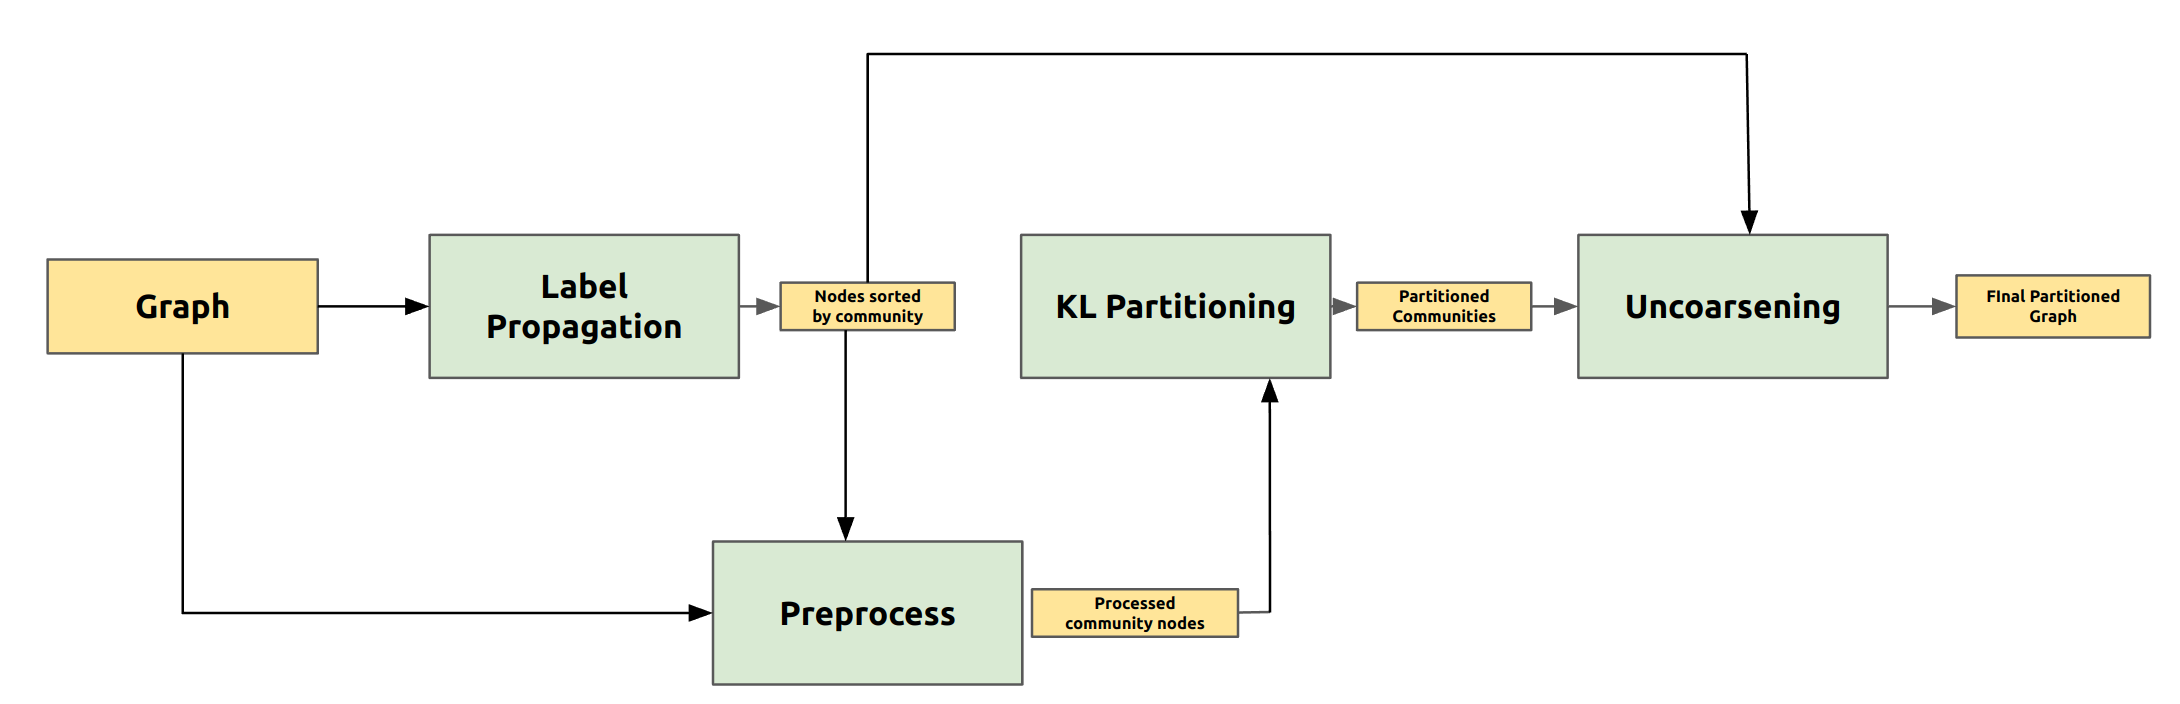
\includegraphics[width=0.9\linewidth]{FIG/full_pipeline.png}
    \caption{Full Pipeline of Our Approach}
    \label{fig:full_pipeline}
\end{figure}

Before we move on to explaining the baselines for coarsening phase, that is, detecting communities, we first show our evaluation metrics. Next, we elaborate on our proposed method in detail.
\subsection{Evaluation Metrics}
\textbf{1. Modularity} \\ \\
Graph modularity is a quality function to evaluate the compactness of communities.\\
The modularity Q is defined as:
\[ Q = \frac{1}{2m}\sum_{ij}^{}\left(A_i_j-\frac{k_ik_j}{2m}\right)\delta\left(s_i,s_j\right)\]
where $2m$ is the volume of edges, $A$ is the graph adjacency matrix, $k_i$ and $k_j$ are the edges of node $i$ and node $j$, $s_i$ and $s_j$ are the community indicator.
Modularity illustrates the difference between the actual number of edges and the expected number of edges for every pair of nodes in one community.\\
A graph is said to be modular if there exists a highest density of edges inside a community and a low density of edges between different communities. 
And as modularity can range from 0 to 1, we can interpret that higher value of Q (closer to 1) means stronger community structures. \\

\subsection{Baseline for Community Detection}
We set our baseline as the three existing community detection algorithms below. For these algorithms we used the implementation of Python library \texttt{communities} in our experiments. \\ \\
\textbf{1. Louvain Algorithm}\\ \\
Louvain algorithm gathers similar nodes or communities together into bigger clusters in the way that greedily maximizes the modularity. One pass is consisted of two phases. In phase 1, for each randomly ordered node, it is removed and inserted in a different community until no significant increase in modularity is verified. In phase 2, all nodes belonging to the same community are merged into a single giant node. \\
This method is widely used for large real world graphs. Although Louvain algorithm simplifies the process of obtaining modularity and runs in $O(nlogn)$ time, $n$ meaning the number of nodes, the calcuation of the modularity occurs every time each node is moved to a different community which leads to long computation time.\\ \\
\textbf{2. Girvan-Newman Algorithm}\\ \\
As a top-down approach, Girvan-Newman algorithm repeatedly removes 'bridge' edges with high betweenness centralities to produce more connected components, or communities. The iteration of the removal of edges terminates when the modularity value no longer increases.Edge betweenness centrality is the number of the shortest paths that go through a certain edge in the given graph. This centrality $c_{B}(e)$  is defined as \[ c_{B}(e) =  \sum_{i,j}^{}  \frac{ \sigma (i,j | e)}{\sigma(i,j)} \] where $\sigma (i,j)$ is the number of shortest paths from node \textit{i} to \textit{j} and $\sigma (i,j | e)$ is the number of shortest paths that pass through edge e.\\
The method runs in $O(m^{2}n)$ time, where \textit{m} is the number of edges and \textit{n} is the number of nodes.\\ \\
\textbf{3. Spectral Clustering}\\ \\
This method makes use of eigenvectors and eigenvalues of the adjacency matrix of the input graph to figure out the community structure. Skipping the first eigenvector, a matrix V is created which contains eigenvectors $v_{1}$, $v_{2}$, ... ,$v_{n}$ as columns. Next, the rows in matrix V are clustered using k-means into k-communities. \\
This is a NP-hard algorithm, which implies that it is unlikely to be applied on large graphs.\\

\subsection{Community detection for reducing the size of RWG} \\
Since real world graph data is huge, reducing the number of vertices of the original graph is needed. We thought that reducing the time complexity of baseline methods into nearly linear time will improve the efficiency of the overall multilevel graph partitioning. The main idea of this approach is iteratively change the label of a node based on the labels of the surrounding nodes. In this way, we can reduce the running time of the algorithm in contrast to the baseline methods, which have to compute the modularity value every iterations. \\


% Label Propagation 알고리즘
\begin{algorithm}
\caption{Label Propagation}
\label{label propagation}
\begin{algorithmic}[1]
\Procedure{Label Propagation}{$G$}
    \State Initialize the labels uniquely at all nodes in the Graph.  
    \State $t = 1$
    \State Make a list X of nodes in random order and set it to X.
    \For {each node $x$ in $X$}
        \State $C_x(t) = f(C_{x1}(t),...,C_{xim}(t),C_{xi(m+1)}(t-1),...,C_{xik}(t-1))$ 
        \State where $f$ returns the highest frequency label of neighbor nodes.
	\EndFor
	\If{Every node has their neighbors' maximum frequency label,} stop
	\ElsIf {Set $t = ${t+1} and go back to line 4} end if
\end{algorithmic}
\end{algorithm} \\

Shown in Algorithm 1, the runtime of the algorithm takes nearly linear time. Initializing all the nodes into unique labels takes $O(n)$ time, where n is the number of nodes. For each node x, deciding the label of that node depends on the label of it's neighbors, which is takes $O(d_x)$ since number of neighbors equals degree of that node x. Since this process is repeated iteratively for each node, it takes worst-case time of $O(m)$ for each node, where m is the number of total edges. \\


\subsection{Grouped clusters as the inputs for KL Algorithm} \\ 
KL is a greedy partition algorithm which takes in a graph containing nodes as input and outputs separate subsets that are connected together. The algorithm optimizes the partition by calculating the gain value in an iterative manner.\\
We expect that putting the result of label propagation into the input of Kernighan-Lin (KL) will elaborate the partitioned result and improve the accuracy of our overall pipelined algorithm.


% KL알고리즘
\begin{algorithm}
\caption{Kernighan-Lin}
\label{kernighan-lin}
\begin{algorithmic}

\Procedure{Kernighan-Lin}{$G$($V$,$E$)}
    \State This algorithms returns $G$($V$,$E$)
    \While{$g_{max} \leq 0$}
        \State $A1 :=A, B1 :=B$
        \State Compute $D$ values for all in $a$ in $A1$ and $b$ in $B1$
        %\State Let $gv, av, bv$ be empty lists
        \For {$i :=1$ to $|V|/2$}
            \State find $a[i]$ from $A1$ and $b[i]$ from $B1$, such that
                \State $g[i] = D[a[i]] + D[b[i]] -2c[a[i]][b[i]]$ is maximal
            \State remove $a[i]$ and $b[i]$ from further consideration in this pass
            \State update $D$ values for the elements of $A1 = A1 / a[i]$ and $B1 = B1 / b[i]$
        \EndFor
        \State Find $k$ which maximizes $g_{max}$, the sum of $g[1],...,g[k]$
        \If{$g_{max} > 0$} {Exchange $a[1],a[2],...,a[k]$ with $b[1],b[2],...,b[k]$}\EndWhile
\end{algorithmic}
\end{algorithm}



\section{Experiments}
    \label{sec:experiments}
    
In this section, we experimentally evaluate our algorithms and compare them to recent multilevel graph partitioning algorithms.
We design experiments to answer the following questions:
\begin{enumerate}
  \item How do the presented algorithm for detecting community system, which previously haven't been well-benchmarked, compare to existing algorithms in terms of time complexity and modularity? 
  \item Our pipeline compared to the baseline on Execution Metrics. 
  \item Our pipeline compared to the baseline on Partition Metrics. 
\end{enumerate}
\subsection{Execution Metrics}
Execution metrics are the type of metrics that can be calculated after processing the graph. Some examples of execution metrics can include processing time, number of rounds performed by the partitioner, partitioning time, and network communication overhead. These types of metrics can help measure on specific applications and execution environments but are not suitable for general comparisons. Another limitation can be that they are very costly to measure and evaluate. 

\subsection{Partitioning Metrics}
From the limitations from the execution metrics stated in the section above, another category of metrics is known as the partition metrics. These types of metrics allow us to evaluate the quality of partitions produced prior to actual graph processing. These metrics are suitable for general comparison and are less costly to evaluate and measure. The most common metrics are the four partition metrics; Balance, Vertex Cut, Largest Partition, and Normalized Standard Deviation. \\ \\
Balance(Bal) is used to measure the ratio between maximum number of edges in one partition and average number of edges in all subsets. It is defined as: \\\\
\begin{equation} \label{eu_eqn}
Bal = \frac{max_(i=1..N)(|E_i|)}{|E|/N}
\end{equation}
\\\\
A cut is a partition of the vertices of a graph into two disjoint subsets. Any cut determines a cut-set, the set of edges that have one endpoint in each subset of the partition. Edge cut determines the number of cutted edges after partitioning, it is defined as: \\\\
\begin{equation} \label{eu_eqn}
EC = |E| - \sum_{i=1}^{N} |F(E_i)|
\end{equation}
\\\\
Largest Partition (LP) is used to show the number of verticies in the largest subset. It is defined as: 
\begin{equation} \label{eu_eqn}
LP = max_(i=1...N) |(E_i)|
\end{equation}
\\
\\
Normalized standard deviation(NSD) is used to show the standard deviation of a partition size. It is defined as:
\begin{equation} \label{eu_eqn}
NSD = |V| - \sqrt{(\sum\frac{|E_i|}{E/N}-1)^2} \frac{1}{N}
\end{equation}
\\\\
We will be using these partitioning, execution metrics for evaluating our pipeline on real world graph partitioning. 

\subsection{Community Detection Experiments}
Community detection is used for coarsening the large real world graph in order to reduce the run time of our partitioning algorithm. Different community detection algorithms already exist, with individual advantages and disadvantages. We ran the following tests to find the optimal coarsening method.
\\ \\ 
The test is ran on the Stanford Large Network Dataset(SNAP), especially on the social networks ego-Facebook; 50,515 Nodes, 819,306 Edges, ego-GPlus; 107,614 Nodes, 13,673,453 Edges, and the munsae-github dataset; 37,700 Nodes, 289,003 Edges. These graphs are all undirected graphs with as many as a million edges and ten-thousand nodes. We chose the most frequently used community detection algorithms; Louvain, Girvan-Newman, Spectral Clustering, and the label propagation algorithm. Table 2, 3, 4 shows the results on each dataset. Note that results that are marked as NA took longer than 3 days and discluded from the results. 
\begin{table}[H]
\centering
\caption{Musae-Github Dataset}
\label{t1}
\begin{tabular}{|c|c|c|c}
\noalign{\smallskip}\noalign{\smallskip}\hline
& Running Time(s) & Modularity(Q)\\
\hline
Louvain & 319.183 & 0.26429\\
\hline
Girvan-Newman & 9283.192 & 0.21029 \\
\hline
Spectral Clustering  & NA & NA \\
\hline
Label Propagation  & 34.291 & 0.24628 \\
\hline
\end{tabular}
\centering
\caption{Ego-Facebook Dataset}
\label{t1}
\begin{tabular}{|c|c|c|c|}
\noalign{\smallskip}\noalign{\smallskip}\hline
& Running Time(s) & Modularity(Q)\\
\hline
Louvain & 494.060 & 0.23912\\
\hline
Girvan-Newman & 15928.182 & 0.19392 \\
\hline
Spectral Clustering  & NA & NA \\
\hline
Label Propagation  & 73.2039 & 0.21293 \\
\hline
\end{tabular}
\centering
\caption{Ego-Google Dataset}
\label{t1}
\begin{tabular}{|c|c|c|c|}
\noalign{\smallskip}\noalign{\smallskip}\hline
& Running Time(s) & Modularity(Q)\\
\hline
Louvain & 71195.620 & 0.36128\\
\hline
Girvan-Newman & NA & NA \\
\hline
Spectral Clustering  & NA & NA \\
\hline
Label Propagation  & 22039.32 & 0.34142 \\
\hline
\end{tabular}
\end{table}

From the results in the tables above, we can confirm that the time complexity of the algorithms are as in the table below.

\begin{table}[H]
\centering
\caption{Running time of community detection algorithms}
\label{t1}
\begin{tabular}{|c|c|c|c}
\noalign{\smallskip}\noalign{\smallskip}\hline
& Time Complexity\\
\hline
Louvain & $O(nlogn)$\\
\hline
Girvan-Newman & $O(m^{2}n)$ \\
\hline
Spectral Clustering & $O(n^{3})$ \\
\hline
Label Propagation  & $O(n)$\\
\hline
\end{tabular}
\end{table}

Modularity is equally important in deciding the optimal community detection algorithm. Although the Louvain's algorithm has the highest modularity value, the difference is minimal leading to our conclusion that it is not suitable to run Louvain for graphs following the power law. Thus, we have decided to select label propagation method, partially giving up the quality in exchange for a faster running time. 
\\
\subsection{Full Pipeline Experiments}
Next we show the results of our full pipeline consisted of Label Propagation for coarsening the graph, partitioning based on the Kernighan-Lin algorithm, and uncoarsening. We are comparing the results to the baseline partitioning algorithms: Fiduccia-Mattheyses, and Kernighan-Lin. Table 7 shows the results on each of the categories of the ego-facebook dataset.
\begin{table}[H]
\centering
\caption{Categories of Ego-Facebook Dataset}
\label{t1}
\begin{tabular}{|c|c|c|c|}
\noalign{\smallskip}\noalign{\smallskip}\hline
& Nodes & Edges\\
\hline
Government & 7,057 & 89,455\\
\hline
New Sites & 27,917 & 206,259\\
\hline
Athletes & 13,866 & 86,858 \\
\hline
Public Figures & 11,565 & 67,114\\
\hline
TV Shows & 3,892 & 17,262\\
\hline
Politician & 5,908 & 41,729 \\
\hline
Artist & 50,515 & 819,306 \\
\hline
Company & 14,113 & 52,310 \\
\hline
\end{tabular}
\end{table}

\begin{table}[H]
\centering
\caption{Evaluation on partitioning metrics: Our pipeline}
\label{t1}
\begin{tabular}{|c|c|c|c|c|}
\noalign{\smallskip}\noalign{\smallskip}\hline
& Balance & Edge Cut & Largest Partition & Normalized Standard Deviation\\
\hline
Government & 1.8392 & 18,923 & 56 & 0.62934 \\
\hline
New Sites & 2.4371 & 135,293 & 269 & 0.78291 \\
\hline
Athletes & 1.5291 & 58,234 & 49 & 0.72819 \\
\hline
Public Figures & 1.8928 & 41,319 & 38 & 0.34912\\
\hline
TV Shows & 1.1293 & 9281 & 21 & 0.22982\\
\hline
Politician & 1.6782 & 27,847 & 46 & 0.68291\\
\hline
Artist & 3.1293 & 682,918 & 48 & 0.81029\\
\hline
Company & 2.1039 & 35,203 & 21 & 0.62731\\
\hline
\end{tabular}
\end{table}
The following tables (Table 8, Table 9) are the experiment results for the Fiduccia-Mattheyses, and the Kernighan-Lin algorithm evaluated with the same metrics. 

\begin{table}[H]
\label{t1}
\centering
\caption{Evaluation on partitioning metrics: Fiduccia Mattheyses}
\label{t1}
\begin{tabular}{|c|c|c|c|c|}
\noalign{\smallskip}\noalign{\smallskip}\hline
& Balance & Edge Cut & Largest Partition & Normalized Standard Deviation\\
\hline
Government & 1.4928 & 17,582 & 43 & 0.82910 \\
\hline
New Sites & 1.8920 & 127,291 & 219 & 0.88392 \\
\hline
Athletes & 1.4192 & 52,019 & 32 & 0.81024 \\
\hline
Public Figures & 1.6718 & 38,742 & 31 & 0.64013\\
\hline
TV Shows & 1.0193 & 7819 & 29 & 0.29301\\
\hline
Politician & 1.5029 & 24,301 & 37 & 0.71902\\
\hline
Artist & 2.8901 & 634,991 & 45 & 0.84059\\
\hline
Company & 1.9841 & 32,049 & 19 & 0.78901\\
\hline
\end{tabular}
\end{table}

\begin{table}[H]
\label{t1}
\centering
\caption{Evaluation on partitioning metrics: Kernighan Lin}
\label{t1}
\begin{tabular}{|c|c|c|c|c|}
\noalign{\smallskip}\noalign{\smallskip}\hline
& Balance & Edge Cut & Largest Partition & Normalized Standard Deviation\\
\hline
Government & 1.6919 & 18,029 & 52 & 0.71894 \\
\hline
New Sites & 2.4019 & 139,401 & 251 & 0.78901 \\
\hline
Athletes & 1.4910 & 56,193 & 58 & 0.69102 \\
\hline
Public Figures & 1.7182 & 46,298 & 49 & 0.51029\\
\hline
TV Shows & 1.1193 & 8689 & 15 & 0.49281\\
\hline
Politician & 1.5890 & 25,291 & 39 & 0.69029\\
\hline
Artist & 2.9103 & 652,948 & 59 & 0.78192\\
\hline
Company & 2.0193 & 32,194 & 18 & 0.78193\\
\hline
\end{tabular}
\end{table}
Now we perform evaluation on the total running time of our pipeline and the baseline algorithms. The running time is measured in seconds(s). We decided that valid results are in the range of maximum two days. Results with NA indicates that the algorithm took more than 3 hours to run on an input graph.
\begin{table}[H]
\label{t1}
\centering
\caption{Running time Comparison(s)}
\label{t1}
\begin{tabular}{|c|c|c|c|c|}
\noalign{\smallskip}\noalign{\smallskip}\hline
& Our pipeline & Fiduccia-Mattheyses & Kernighan-Lin \\
\hline
Government & 18.592 & 159.102 & 468.495\\
\hline
New Sites & 789.192 & NA & NA\\
\hline
Athletes & 49.761 & 278.301 & 1789.301 \\
\hline
Public Figures & 42.982 & 156.693 & 1491.092\\
\hline
TV Shows & 5.119 & 78.103 & 391.982\\
\hline
Politician & 7.992 & 91.592 & 420.678\\
\hline
Artist & 1018.824 & NA & NA\\
\hline
Company & 165.834 & 890.069 & 2782.958\\
\hline
\end{tabular}
\end{table}
Observing the output, we could find that the average running time of our pipeline is approximately \emph{12.56} times faster compared to the Fiduccia-Mattheyses, and \emph{36.78} times faster compared to the Kernighan-Lin algorithm. If the number of nodes of the input graph is larger than 100k, the running time cannot be compared since the baseline algorithms takes too long. We can conclude that by giving up a small amount of quality of the partitioning (compared with edge cuts), we can partition real world graphs much faster. 

\section{Conclusions}
    \label{sec:conclusions}
    This is one of the few papers which focuses on partitioning real world graphs using a multi-level approach. We propose to use a community detection algorithm named label propagation for coarsening, or clustering, the initial nodes to exponentially reduce the running time of our pipeline. The major contributions are listed as follows: 
\begin{enumerate}
  \item Built a multi-level graph partitioning pipeline which can robustly partition graphs with more than 100k nodes.
  \item Used label propagation, a robust community detection algorithm for reducing running time by forming clusters of original nodes. 
  \item Significantly reduced running time of partitioning compared to the previous baselines. 
\end{enumerate}
Label propagation method in the coarsening stage greatly reduces the running time of our overall algorithm. While doing survey and experiments, we verified that label propagation method runs in linear time. Our pipeline is approximately 12 times faster than the Fiduccia-Mattheyses algorithm, and 37 times faster than Kernighan-Lin algorithm. So we assumed that before performing the partitioning stage, using label propagation could improve the overall architecture of partitioning real world graph data in terms of running time of the algorithm. \\ 
By implementing the pipeline that we designed, we could verify that the number of clusters of the output is significantly smaller than the number of clusters in the original graph, while preserving the property of the original graph. Therefore, by applying the KL algorithm to the reduced number of cluster nodes, time consumed in partitioning is much faster. Through the experiments we confirmed that by giving up minimal amount of partitioning quality, we could gain much more running time reduction.\\
Future work could generalize our algorithm for partitioning real world graphs to time evolving real world graphs. 

\newpage
    \bibliography{BIB/other}
    \bibliographystyle{plain}

\newpage
\appendix
\section{Appendix}

\subsection{Labor Division}
The team performed the following tasks.
\bit
\item Survey [all]
\item Partitioning methods study [Hyoyoung Lho]
\item Design of our experiment [Sohyun Kim]
\item Implementation [Yonwoo Choi]
\item Evaluation of the results [Yonwoo Choi]
\item Reports and presentation [Hyoyoung Lho, Sohyun Kim]
\eit

\subsection{Plans of Progress}
\begin{figure}[htb!]
    \centering
    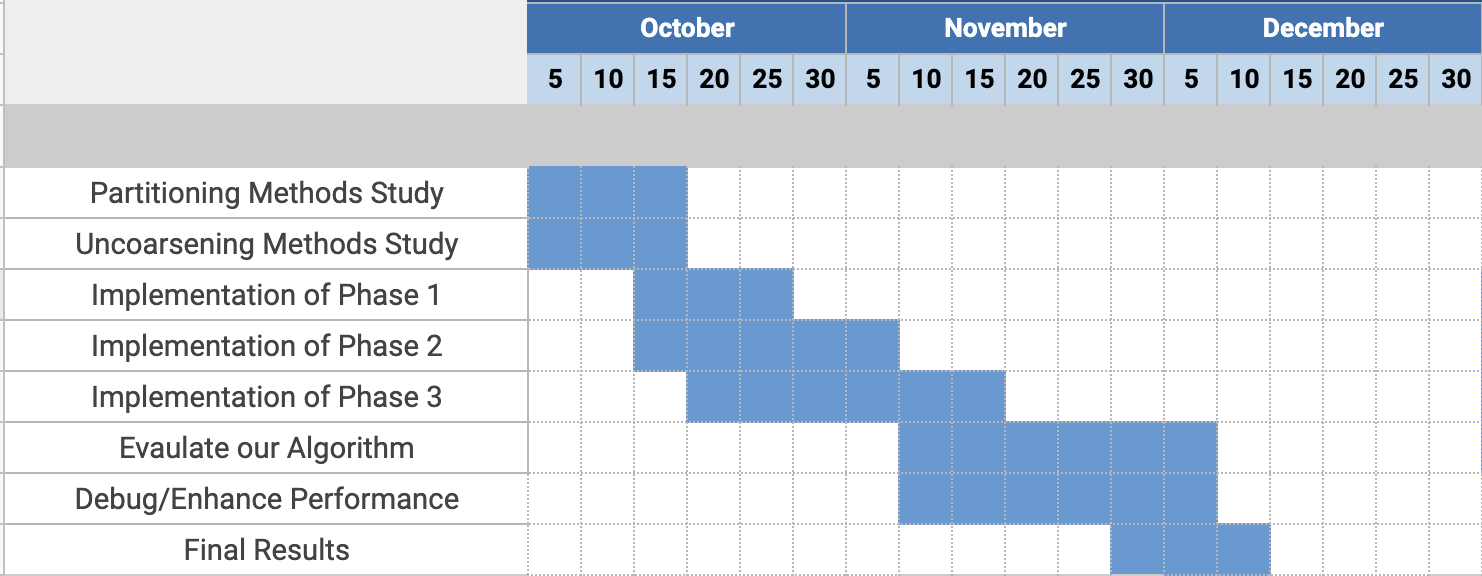
\includegraphics[width=0.9\linewidth]{FIG/ganttchart.png}
    \label{fig:ganttchart}
\end{figure}

\newpage
\subsection{Additional}
\begin{figure}[htb!]
    \centering
    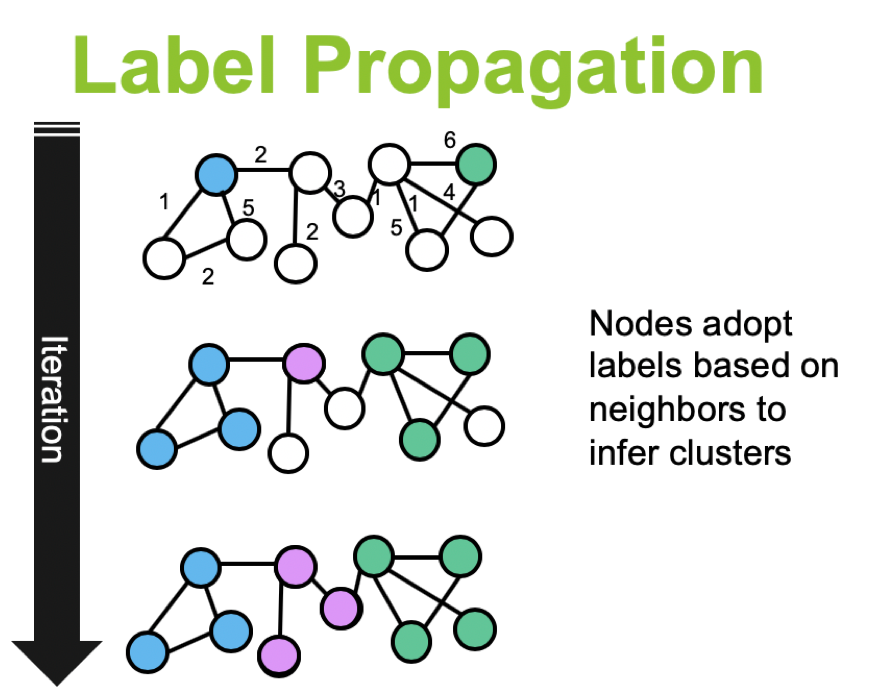
\includegraphics[width=0.5\linewidth]{FIG/lp.png}
    \caption{Label Propagation}
    \label{fig:lp}
\end{figure}

\begin{figure}[htb!]
    \centering
    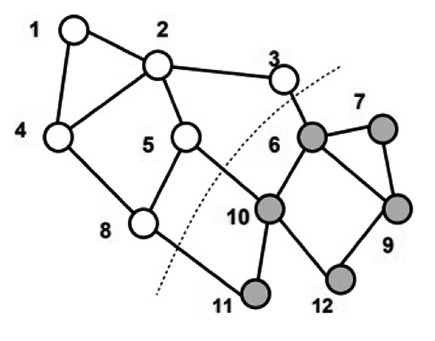
\includegraphics[width=0.5\linewidth]{FIG/kl.png}
    \caption{Kernighan Lin}
    \label{fig:kl}
\end{figure}

\subsection{Full disclosure wrt dissertations/projects}

\paragraph{Choi:} No dissertation related to this project

\paragraph{Lho:} No dissertation related to this project

\paragraph{Kim:} No dissertation related to this project


\newpage
\pagenumbering{roman}
\tableofcontents


\end{document}
